\documentclass[a4paper,12pt]{article}
\usepackage[left=2.5cm,right=2.5cm,top=0cm]{geometry}
\usepackage{tikz}

\usetikzlibrary{shapes.geometric}
\usepackage{hyperref}
\hypersetup{
    colorlinks=false,
    urlbordercolor=white
    }
\usepackage[none]{hyphenat}
\title{Monthly Maths Circle India Challenge}
% \author{Disha Kuzhively}
% \email{disha.jk@icts.res.in}
\date{Solutions\\February 2024}
\begin{document}
\maketitle
\thispagestyle{empty}
\begin{enumerate}
    \item[Solution 1.] We can divide Bindu's trapezium into four triangles. The triangles $B_1$ and $B_2$, which form two of the arms of the star, are each congruent to Anita's triangles $A_1$, $A_2$, and $A_3$. Triangle $B_3$ is congruent to $B_2$, and triangle $B_4$ is congruent to $A_4$.

    \begin{figure}[h]
        \centering
        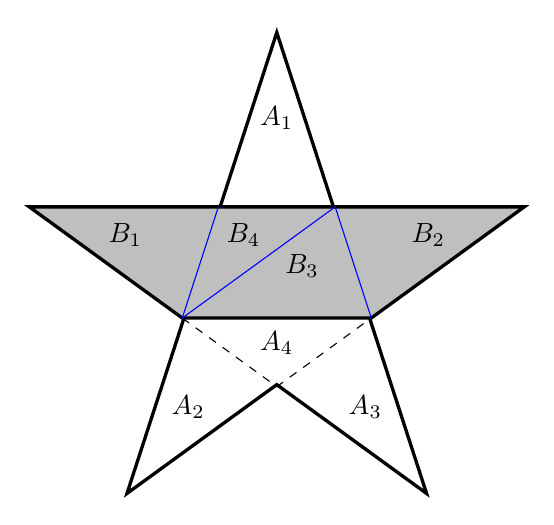
\begin{tikzpicture}
    \def\radius{1cm}
    \def\factor{1/cos(72)}
    \def\infactor{1/cos(36)}
\node [name=s, shape=star, star points=5, star point height=\radius*(\factor-\infactor), minimum size=2*\radius*\factor, draw,very thick] at (0,0) {};
\filldraw[fill=gray!50,very thick, draw=black] (s.inner point 2) -- (s.inner point 4) -- (s.outer point 5) -- (s.outer point 2) -- cycle; 
\draw[dashed] (s.inner point 2) -- (s.inner point 3) -- (s.inner point 4);
\draw[blue] (s.inner point 1) -- (s.inner point 2) -- (s.inner point 5) -- (s.inner point 4);
\node[below, inner ysep=1cm] at (s.outer point 1) {$A_1$};
\node[above right, inner ysep=1cm, inner xsep=0.6cm] at (s.outer point 3) {$A_2$};
\node[above left, inner ysep=1cm, inner xsep=0.6cm] at (s.outer point 4) {$A_3$};
\node[above, inner ysep=0.4cm] at (s.inner point 3) {$A_4$};
\node[below right, inner ysep=0.2cm, inner xsep=1cm] at (s.outer point 2) {$B_1$};
\node[below left, inner ysep=0.2cm, inner xsep=1cm] at (s.outer point 5) {$B_2$};
\node[below left, inner ysep=0.6cm, inner xsep=0.2cm] at (s.inner point 5) {$B_3$};
\node[below right, inner ysep=0.2cm, inner xsep=0.1cm] at (s.inner point 1) {$B_4$};
\end{tikzpicture}
                
    \end{figure}

    The total area of Anita's four triangular cakes is indeed equal to the area of the single large trapezium cake baked by Bindu. Therefore, the cost should be split equally between the two.

    \textit{The best solution to this problem was sent to us by Ahona Mukherjee}
    
    \item[Solution 2.] We can construct a square of area 5 by constructing $\sqrt{5}$. On the square grid, this would be the hypotenuse of the right triangle with sides of lengths 1 and 2. See the figure below.
    \begin{figure}[h]
        \centering
        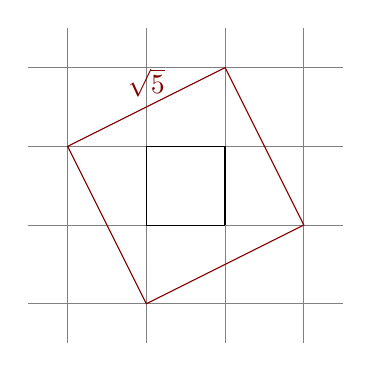
\begin{tikzpicture}
    \draw[gray] (-1.5,-1.5) grid (2.5,2.5);
    \draw[black] (0,0) grid (1,1);
    \draw[red!50!black] (-1,1) -- (1,2) node[midway, above]{$\sqrt{5}$} -- (2,0) -- (0,-1) -- cycle;
    % \node [fill=red,inner sep=1pt,label=below:$X$] (X) at ($ (A)!.5!(B) $) {};
    \end{tikzpicture}
    \end{figure}
\end{enumerate}
\end{document}